\section{Finding Clusters} \label{sect:finding}

Finding aggregate catchments --- pools of clients essentially directed toward
the same web resources --- necessarily involves finding sets of clients with high
CNRE measures between each other. Because CNRE is a measure of similarity, this
problem naturally lends itself to hierarchical clustering techniques \cite{murtagh1983survey}. 
We employ the complete linkage method to ensure cluster formation reflects commonalities
across all cluster members as opposed to potentially edge-specific properties.
Note that in all \emph{clustering} calculations, we opt to use the CNRE \emph{distance}
as defined in Section \ref{sect:cnre}.

Establishing heirchical clusters requires that we have some definition of what
constitutes a \emph{high} or \emph{low} CNRE measure and at what threshold it is
appropriate to consider clients sufficiently similar such that they appear in
the same cluster. In this section, we explore the implications of various CNRE
values, as well as CNRE's relationship with other, well-established client grouping
systems: country, ASN, BGP prefix, and /24 prefix subnet.

\begin{figure*}
    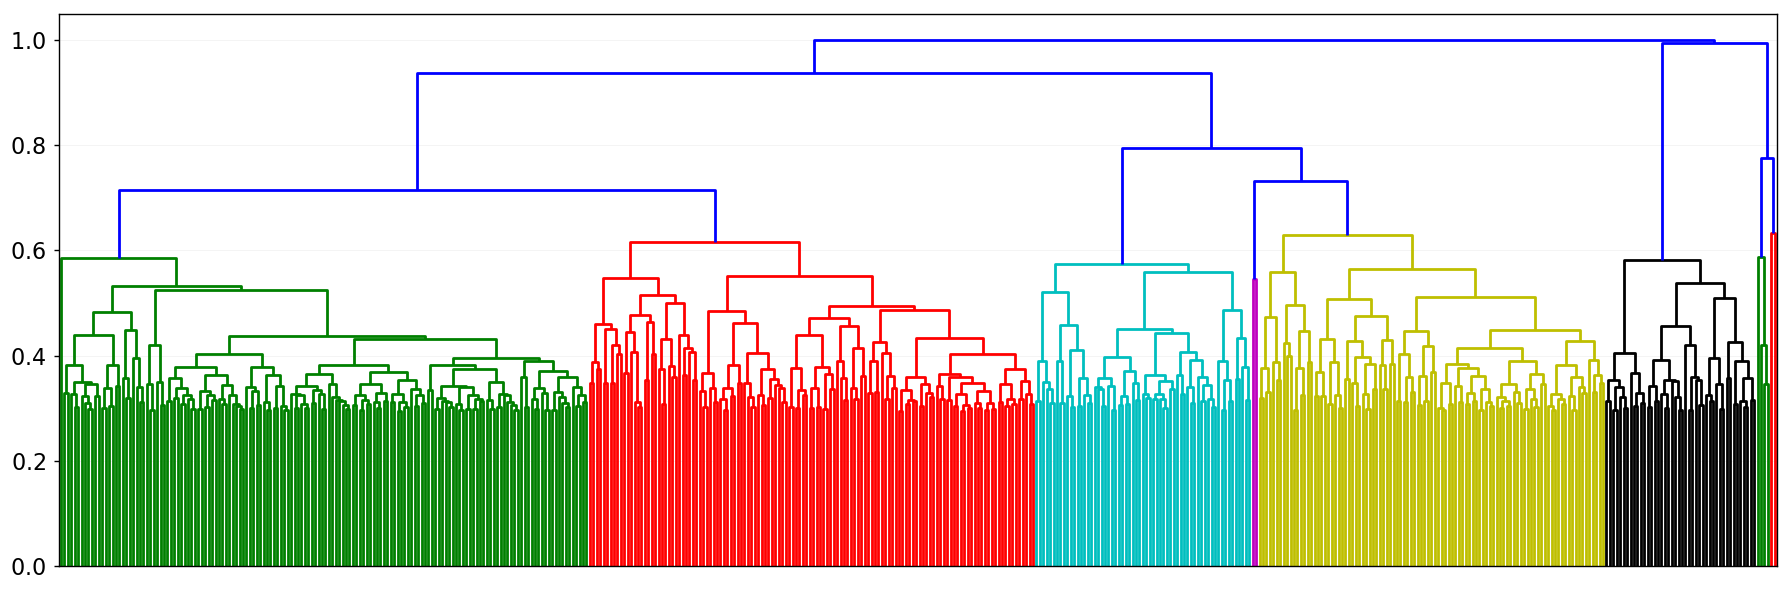
\epsfig{file=figs/dendrograms/v0.png, width=1\linewidth}
    \caption{Dendrogram of CNRE distance across all client pairs}
\end{figure*}


\begin{figure*}
    \center
        \mbox{
            \begin{subfigure}[b]{0.33\linewidth}
                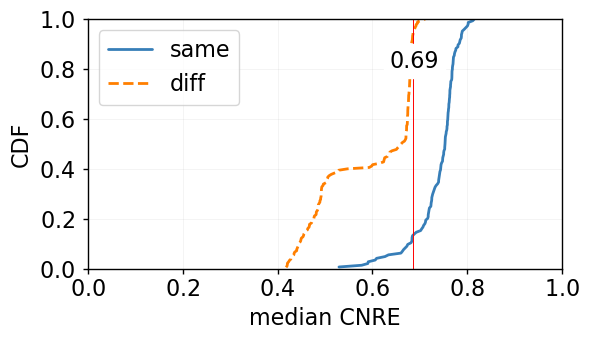
\epsfig{file=figs/cnre_vs_category/country.png, width=1\linewidth}
                \caption{country} 
            \end{subfigure}
            \begin{subfigure}[b]{0.33\linewidth}
                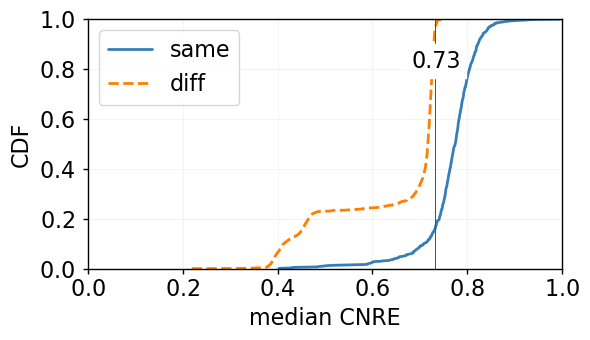
\epsfig{file=figs/cnre_vs_category/asn.png, width=1\linewidth}
                \caption{ASN} 
            \end{subfigure}
            \begin{subfigure}[b]{0.33\linewidth}
                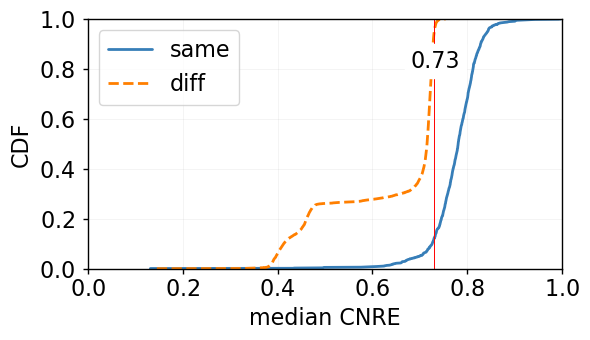
\epsfig{file=figs/cnre_vs_category/prefix.png, width=1\linewidth}
                \caption{BGP prefix} 
            \end{subfigure}
        }
    \caption{CDFs of CNREs across client sets with matching (same) and non-matching (diff) labels. 
    ``Same'' shows the CDF for the median CNRE distance across all client pairs matching a given label. 
    ``Diff'' shows the CDF for the median CNRE distance from each label group toward all other labels.}
    \label{fig:vslabel}

\end{figure*}


 Figure \ref{fig:vslabel}


\begin{figure}
    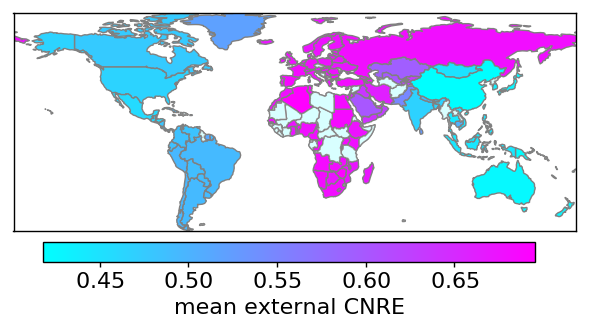
\epsfig{file=figs/cnre_country_uniqueness_map.png, width=1\linewidth}
    \caption{Choropleth with each country shaded by its median CNRE distance from all other countries. TODO: add legend (I'm struggling to format it in geopandas...)}
\end{figure}

\begin{figure*}
    \center
        \mbox{
            \begin{subfigure}[b]{0.33\linewidth}
                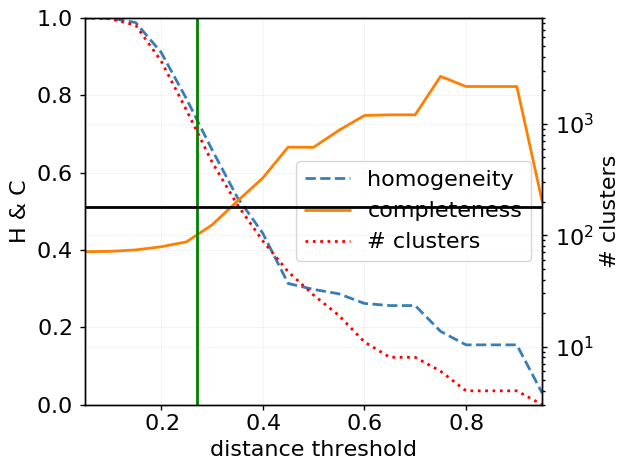
\epsfig{file=figs/completeness_vs_homogeneity/country.png, width=1\linewidth}
                \caption{country} 
            \end{subfigure}
            \begin{subfigure}[b]{0.33\linewidth}
                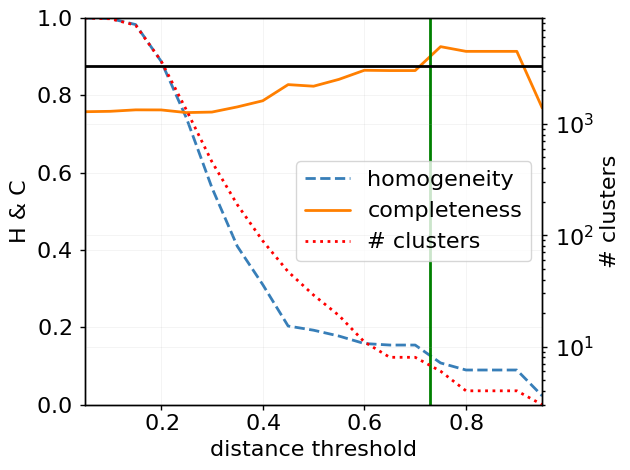
\epsfig{file=figs/completeness_vs_homogeneity/asn.png, width=1\linewidth}
                \caption{ASN} 
            \end{subfigure}
            \begin{subfigure}[b]{0.33\linewidth}
                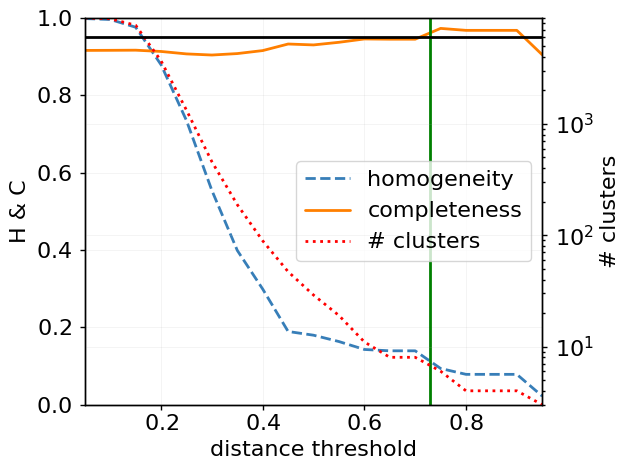
\epsfig{file=figs/completeness_vs_homogeneity/prefix.png, width=1\linewidth}
                \caption{BGP prefix} 
            \end{subfigure}
        }
    \caption{Completeness and homogeneity (for each feature) vs clustering distance threshold. The vertical line marks 0.73, the CNRE distance at which clients with different labels become distinguishable.}
\end{figure*}
